\documentclass[11pt]{article}

% Generated by paper/score/build/build.py from paper/score/source/score.md. Do not edit.
\usepackage{iftex}
\ifPDFTeX
  \usepackage[T1]{fontenc}
  \usepackage[utf8]{inputenc}
  \usepackage{lmodern}
  \usepackage{textcomp}
\else
  \usepackage{fontspec}
\fi
\usepackage{amsmath,amssymb}
\usepackage{longtable,booktabs,array,calc}
\usepackage{graphicx}
\usepackage{xcolor}
\usepackage[numbers,sort&compress]{natbib}
\usepackage{microtype}
\usepackage[margin=2.5cm]{geometry}
\usepackage[colorlinks=true,linkcolor=blue,citecolor=blue,urlcolor=blue]{hyperref}
\providecommand{\tightlist}{\setlength{\itemsep}{0pt}\setlength{\parskip}{0pt}}
\providecommand{\pandocbounded}[1]{#1}
\setlength{\emergencystretch}{3em}

\title{SCORE: Synthesising Complete, Owned, Responsive Environments for
Simulation}
\author{J.P. Kardolus, Babon Innovations B.V., Utrecht, The Netherlands}
\date{Working draft, 17 November 2026}

\begin{document}
\maketitle
\begin{abstract}
Simulation needs worlds that a physics engine can step: separate objects
with mass, colliders and joints, a consistent look, and people whose
bodies obey the same physics. World generation models now produce
convincing pictures, videos and splats of places, yet none of them
delivers such a scene, and none hands its creator a file to own and
edit. SCORE is an open framework that closes this gap by composing the
best current commercial and open-source models around two open
foundations, OpenUSD for the scene and MuJoCo for its physics. A
creator's concept picture is segmented into objects, the missing objects
are generated, every object is finished from one shared library, the
assembled scene is checked in simulation, and people are added as
musculoskeletal bodies solved by MOTOR. Four places built this way pass
every physical check and are written as OpenUSD stages that their
creator owns and can edit. Code:
https://github.com/Babon-Innovations-b-v/score (MIT).
\end{abstract}


\makeatletter\def\fps@figure{tp}\makeatother\renewcommand{\topfraction}{0.9}\renewcommand{\textfraction}{0.1}

\begin{figure}
\centering
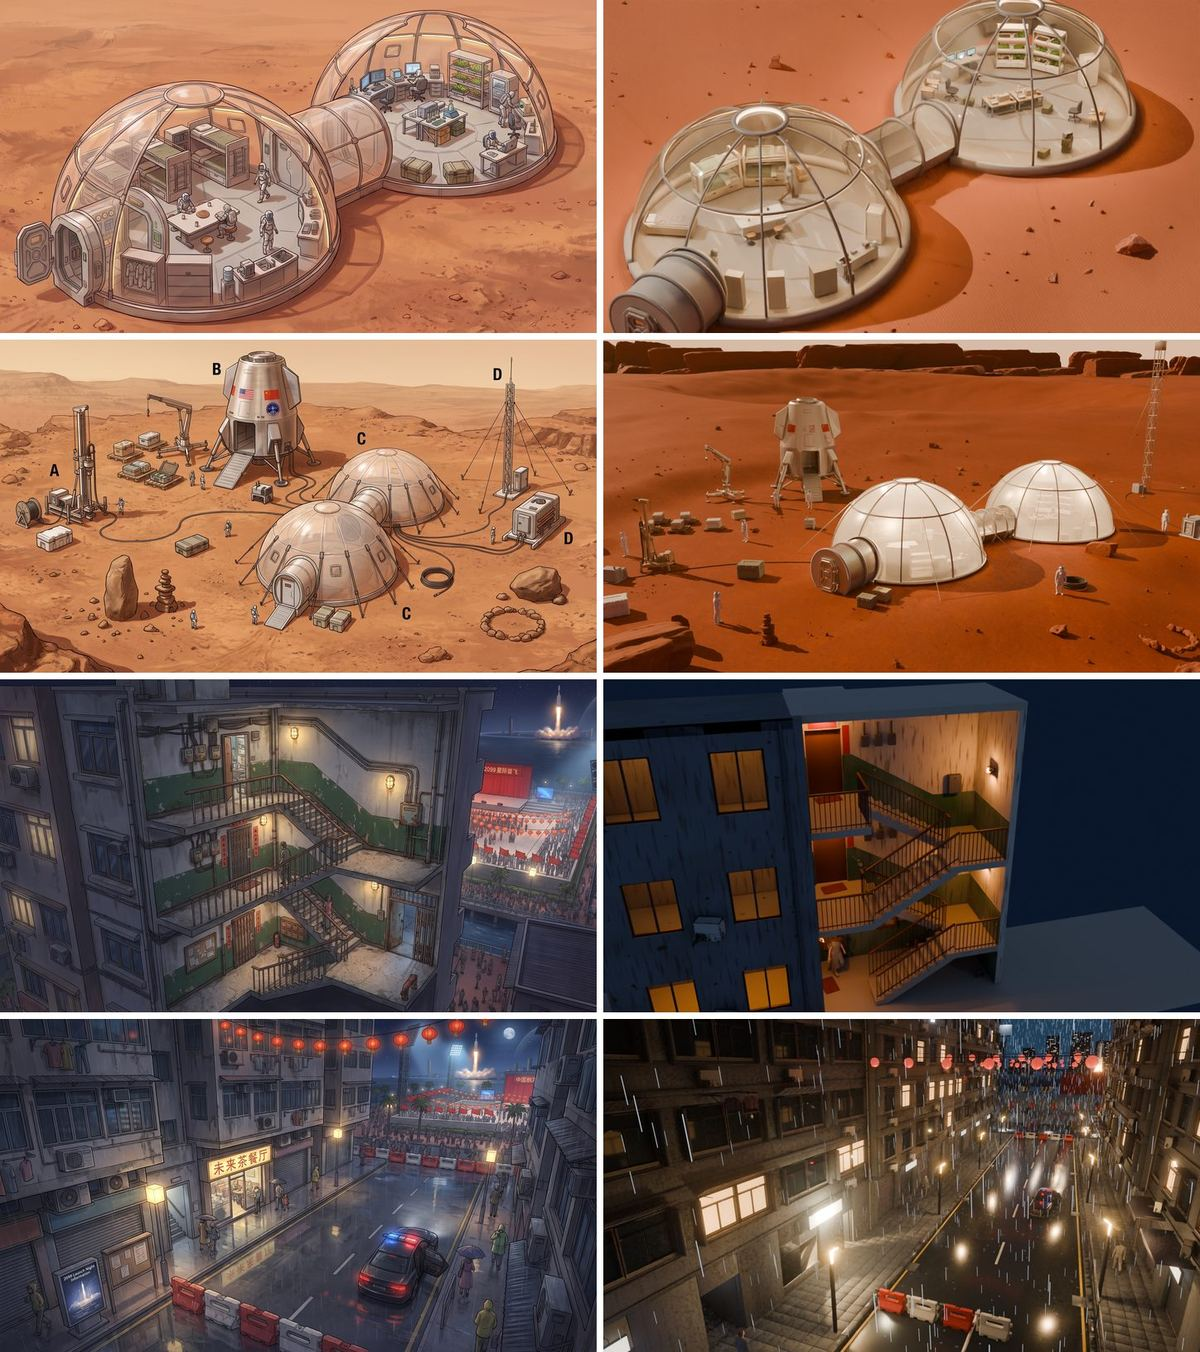
\includegraphics[width=1\linewidth,height=\textheight,keepaspectratio,alt={Each place's locked concept (left) beside the final render of its scene from the concept's own view (right): camp, campgrounds, stairwell and street, top to bottom. Every object in the renders is a library entry laid by the placing agent, and every scene passes the physics-readiness check with no fault.}]{figures/places.jpg}
\caption{Each place's locked concept (left) beside the final render of its scene from the concept's own view (right): camp, campgrounds, stairwell and street, top to bottom. Every object in the renders is a library entry laid by the placing agent, and every scene passes the physics-readiness check with no fault.}
\end{figure}

\section{Introduction}\label{introduction}

Simulated 3D environments serve games, film, robot learning and embodied AI \citep{yang2024holodeck}. Across these uses they share a common structure of separate objects with collision geometry and mass, a ground with its gravity, light from identifiable sources, and scenes that can be reopened, modified and simulated again. Authoring such an environment by hand is expensive, and a generative system that takes over this work must leave the result in the hands of its author, since in the Game Developers Conference's 2026 survey 52 percent of game workers considered generative AI to be harming the industry \citep{gdc2026survey}.

World models generate an environment as a sequence of video frames \citep{bruce2024genie, genie3} that no physics simulator can step forward in time. 3D environment generators \citep{wang2025worldgen, hyworld2} produce geometry, mostly as a single fused asset from which separate objects have to be recovered afterwards \citep{hu2026worldact, niu2026worldsculpt}. Procedural systems \citep{raistrick2023infinigen, raistrick2024indoors} and coding agents that write scenes as executable programs \citep{hu2024scenecraft, li2026rcwm, guo2026worldclaw, yin2026autoue, he2026thinking, wang2026codeasworlds} keep the environment explicit and inspectable, but the models they produce often float above their supports or come apart \citep{gao2026codebench3d}, and such agents assess their own geometry unreliably \citep{li2026lego}. Open vision foundation models now recover segmentation masks \citep{carion2025sam3} and 3D shape \citep{li2026pixal3d, xiang2024trellis, trellis2} from single images, and a coding agent can call them as tools, yet none of them provides physical properties, and objects made by different models rarely share one visual style \citep{wu2026production, yang2026flowscene}.

The components needed for the physics already exist. OpenUSD \citep{openusd}, the scene description that Pixar developed for film production, composes scenes from smaller ones by reference and describes rigid bodies, colliders and mass in the same stage, and MuJoCo \citep{todorov2012mujoco} is a widely used engine for bodies in contact. What is missing is a route from what a creator intends, typically a single concept picture, to a complete environment in this form that still reads as that picture.

SCORE is a framework for that route. Its environments are complete, since every object, surface and light a scene shows exists wherever the viewer looks; owned, because every model in the framework permits commercial use of its output and every object comes from the creator's own asset library, score\_lib; and responsive, because every object carries its collider, mass and material, so a simulator steps the environment as written. This paper reports a change of method. SCORE's first method derived every scene from its concept through a chain of model readings, written plans and generated shells. Measured on 26 places of a first environment, that derivation produced scenes far from their concepts (Section 2). We replaced it with kit placement (Section 3): an agent lays library pieces, renders the concept's own view, compares and corrects, under a physics-readiness check that refuses any scene a simulator could not step. People are then routed through the checked floor and given musculoskeletal sim bodies (Section 4). Section 5 reports four places built this way, with their scores against the concepts, their checks, their walkers and their costs, and Section 6 states what still fails.

\section{Why the per-picture derivation failed}\label{why-the-per-picture-derivation-failed}

The first method turned each locked concept into a scene in stages, each one a model call or a rule. Gemini 3.1 Pro \citep{gemini31pro} listed every object of the concept as a row of a scene inventory, and SAM 3 \citep{carion2025sam3} localised each row with a box. A plan in metres was then written from a drawing of the scene from above, a scene record built shells, stairs and ground from that plan, every inventory row became a model made from a close-up of its crop, and an assembly placed the models by rules on what holds what. Every stage passed measured checks before the next began, and paid stages were bought in phases.

The method was carried to stills of all 26 places of the first environment. Reviewing agents then scored each still against its concept and traced every shortfall to its cause. The mean was 2.2 out of 10, the best place reached 4, and no place read as its concept. The individual models were often fair; what failed was the scaffolding between them. Room outlines, heights and shapes came from the written plan rather than from the concept and were wrong in 18 places, partly because the shell builders could not make several shapes the concepts draw, such as a dome with a rise, a round tube or a sunken pit. Walls, frames, panels and terrain named in the inventory produced no geometry, so most walls were a single flat finish. Fitting a model into its box scaled it by its tightest side, which shrank doors and furniture in 17 places. The reading dropped key objects and doubled others, and each duplicate door cut another opening into a wall. Placement followed generic rules rather than the relations the concept shows, so tunnels were pushed apart from the domes they join and copies were lined up along one wall. Several of these faults cannot be repaired by rules, because a layout read from one isometric picture is ambiguous and a written plan and a concept that disagree need someone to decide which one wins.

Eight rounds of fixes over the following night, about 40 commits, did not change the picture: the creator judged the reworked previews no better and stopped the run. Each fix also re-keyed paid outputs, so that re-buying the 77 paid rows the first rework round touched alone would have cost EUR 85.65. The creator decided to change the method rather than patch its rules, to build fewer places properly, and to remove the per-picture chain (the inventory reading, the plan writing and its fixes, the scene record, the shells and the assembly) once its usable content had been moved into score\_lib.

\section{Method: placing a scene from its concept}\label{method-placing-a-scene-from-its-concept}

\subsection{The concept and its objects}\label{the-concept-and-its-objects}

A place begins, as before, with a concept picture the creator has locked. It is no longer read into rows, counts and a plan. SAM 3, run on a local graphics card, segments the whole picture into objects, each with its pixel box, mask and the word that found it, and an instance that duplicates a surer one under another word is dropped. These objects are the placing agent's list of what the scene must contain; how many there are and where they stand is the agent's to read from the picture, checked against the render.

\subsection{Kit placement and the concept-view compare loop}\label{kit-placement-and-the-concept-view-compare-loop}

The scene is built by a coding agent, Claude Code \citep{claudecode}, through one command-line tool, \texttt{place\_build}, whose steps lay and adjust a plain OpenUSD stage in metres. Every object it lays is a score\_lib entry copied whole into the place: modular kit pieces, models, the dome shells and tunnels, a switchback stair core of real size (0.167 m risers and 0.28 m treads), chamfered building blocks with window openings, lamps and sky domes. A surface step binds a library material over an object or one of its parts, so a model's baked colour never shows where the library has a better finish. Many steps run in one process on one open stage, so a complete relayout takes seconds.

The agent then renders the concept's own view, a camera it sets to match the concept's composition, through Blender's Cycles renderer \citep{blender}, and reads the render beside the concept. A review step renders a contact sheet of the same scene in one call: a plan section 2.4 m above the floor with a metre grid and object names, four corner views, eye-height views from each door, close-ups of each compartment, the concept in a corner and any physics fault boxed in red. From these the agent decides the next correction, such as moving a cluster of props to the side of the room where the concept shows them, changing a dome's height, or swapping a model that reads wrongly. Nothing in the tool judges the scene; it only lays, measures and renders, and the loop ends when the render reads as the concept, with the same room, layout, main objects and mood, while details may differ.

\subsection{One library, one palette a place}\label{one-library-one-palette-a-place}

Everything a place shows comes from score\_lib, and the usable content of the earlier method, the models that had passed their checks, its procedural materials and its code-made kits, was moved there before the old stages were removed. Because scans and models from many sources look inconsistent side by side, each place takes in one scene surface library, a set of procedural material variants written as ProcFunc recipes \citep{raistrick2026procfunc} on Infinigen's shaders \citep{raistrick2023infinigen} in the place's palette tokens, with their wear and dirt. Shells, floors and repainted parts take their finishes from it, so that they share the look of the props.

\subsection{Props made with TRELLIS.2}\label{props-made-with-trellis.2}

A prop that the library lacks, or whose model reads worse than the picture, is made with TRELLIS.2 \citep{trellis2}, an open image-to-3D model released under the MIT licence, from a crop of the concept cut out by its SAM 3 mask or from the close-up of an earlier model. The model is generated on the creator's own 16 GB graphics card, built from source with its dependencies at pinned commits, in about three minutes per prop under load. The new mesh is fitted over the model it replaces by quarter turns and one uniform scale, minimising the two-way distance between their point sets. Its own paint is then graded 60 percent of the way toward the nearest palette token, and a colour group that stays far from every token is reported so that the agent can repaint it from the library. Finally the model is made simulation-ready. CoACD \citep{wei2022coacd} decomposes it into convex hulls for collision, its mass is the hulls' outer surface times the material class's sheet thickness and density, and friction and restitution follow the class. On six camp props the masses lie beside those of the earlier models (a crate of 4.0 against 2.6 kg, a desk of 44 against 42 kg, a chair of 5.1 against 4.7 kg), but steel frames come out heavy, because a hull closes over a frame's gaps. Figure 2 compares the two routes on the same pictures.

\begin{figure}
\centering
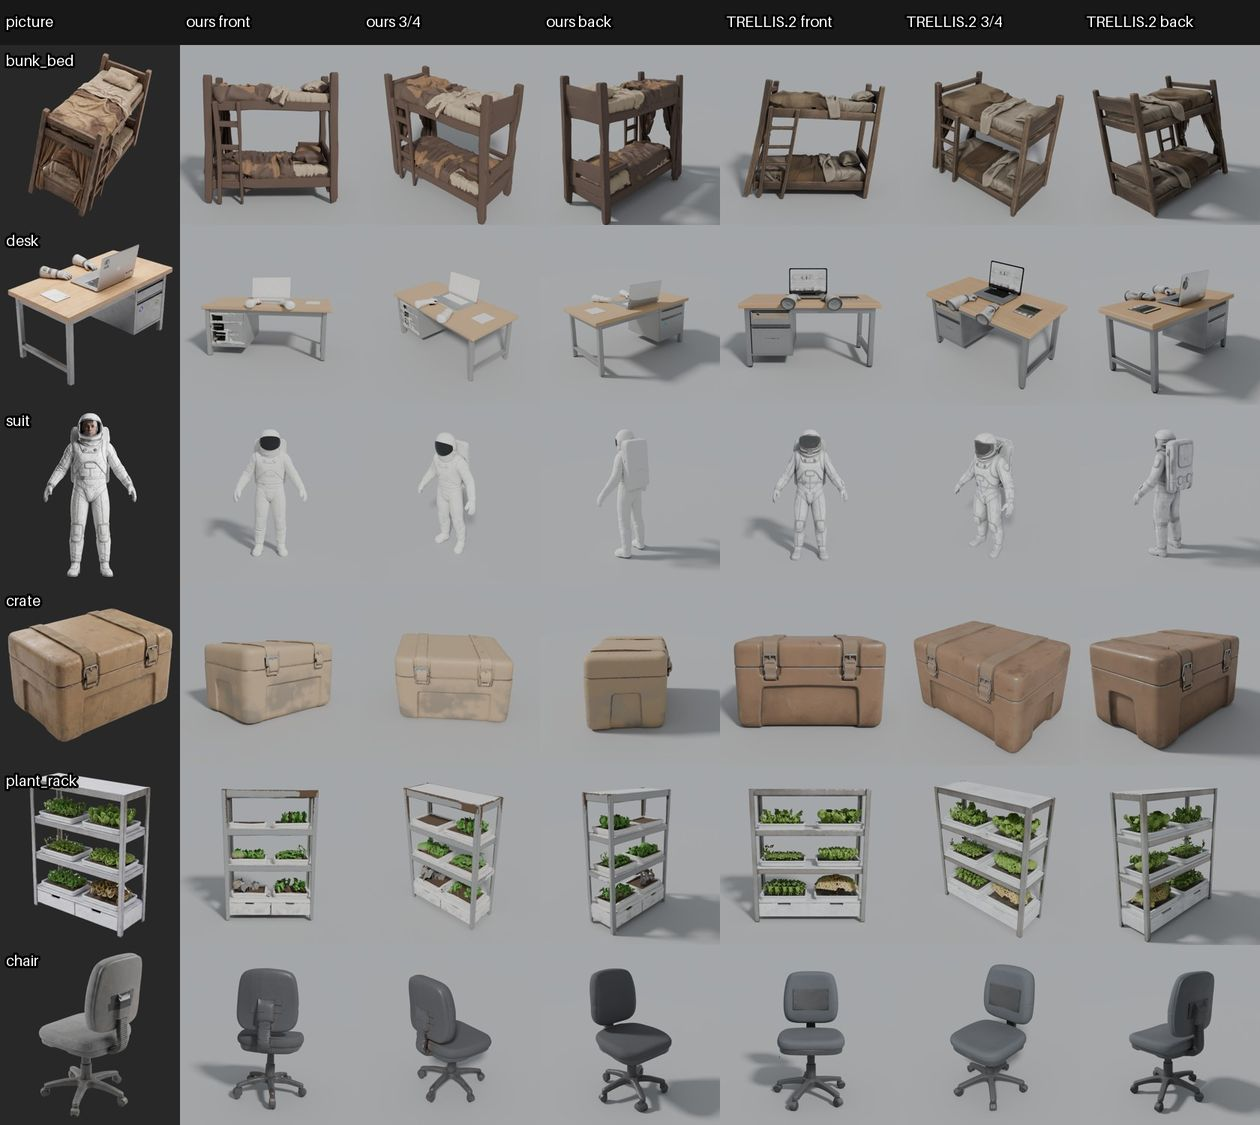
\includegraphics[width=0.88\linewidth,height=\textheight,keepaspectratio,alt={The same six camp pictures (left) made by SCORE's earlier picture-made route (centre three columns) and by TRELLIS.2 (right three columns), each from the front, three-quarter and back. The building agent judged the TRELLIS.2 model the better match on five of the six.}]{figures/trellis2.jpg}
\caption{The same six camp pictures (left) made by SCORE's earlier picture-made route (centre three columns) and by TRELLIS.2 (right three columns), each from the front, three-quarter and back. The building agent judged the TRELLIS.2 model the better match on five of the six.}
\end{figure}

\subsection{Real terrain}\label{real-terrain}

Outdoor places stand on real ground. A terrain entry is a heightfield read from a public-domain digital terrain model of the HiRISE camera on the Mars Reconnaissance Orbiter \citep{mcewen2007hirise} (NASA/JPL/University of Arizona), fetched by range requests rather than as a whole file, dense near the place and sparser toward a horizon that bends with the planet. A building's site is levelled to its laid height and eased into the surrounding relief, and loose rocks are set onto the relief at their own footprints.

\subsection{The physics-readiness check}\label{the-physics-readiness-check}

A scene that reads as its concept may still be one a simulator cannot use, and every round of the compare loop therefore ends with a physics-readiness check. It assigns each object a role from the scene (ground, shell, structure, connector, door, prop, mount, person or far scenery) and reports every fault by object and kind. Each object must rest on a support within 3 cm and stand in balance, and sampled points of its surface must not lie inside another object. A door must lie in an opening, with its outline within 5 cm of the opening's edge, and a connector such as a tunnel must meet the structures it joins within 30 cm with a floor along its length. Every person's feet must touch a floor within 1 cm, and no body may be torn. The walkers' floor is computed as Recast-style walkable spans \citep{recast} with every solid's footprint removed and eroded to a way at least 0.9 m wide, and it must link every spot a walker is sent to. Ground and fixed pieces more than 20 m beyond anything a walker can reach count as scenery and are left out of every measure. Finally, the props are released as free bodies in MuJoCo 3.15 for one simulated second at Earth gravity, one small model per object with its static neighbours, and any prop that falls, tips or drifts is a fault. Every fault kind has a planted counterpart in the check's test, which must be reported by name. The check never moves anything; the agent corrects and runs it again.

\subsection{A builder tournament}\label{a-builder-tournament}

A single agent's layout depends on its early choices, so each place was built by three independent builders that used the same tools, library and check, each trying its own layout. Judging agents compared their concept-view renders with the concept, the best one was kept, and a final builder refined it with the strongest elements of the others. The tournament's per-builder scores were not kept as a record; only the winning scenes and their checks were.

\section{People in the place}\label{people-in-the-place}

\subsection{Routes and joined motion}\label{routes-and-joined-motion}

Each walker is given spots to pass through and the length of its film. Its route is the shortest way through those spots over the check's own walkers' floor, with doors open as passages and a stair flight as a run of spans one riser apart, its corners kept by line of sight and rounded over 0.6 m, so a route never leaves floor the check has judged. A walker that must fill its film walks on around its spots until it does. The route is then timed at 1.0 m/s on the flat and one tread per step on a flight, eased from standing at the start and back to standing at the end, and cut into pieces of at most 7 s at every start and end of a flight. Each piece is generated by Kimodo \citep{rempe2026kimodo} in its own canonical frame from the dense path and heading of its stretch, as a flat walk or as a climb with each foot asked onto its tread. Every piece after the first is constrained by full-body keyframes on its first four frames to the pose in which the previous piece stood there, so that position and velocity match across the join. The pieces are joined back in the scene's frame by blending over those shared frames, with the standing foot held on its spot. The travel therefore comes from the clips themselves; a clip is never slid, stretched or looped along a line. Each walker is measured against fixed limits: foot skate per stance of at most 2 cm, the hips within 10 cm of the route, and the body clear of every upright solid between knee and head.

\subsection{Sim bodies and the peel}\label{sim-bodies-and-the-peel}

Every walker also receives a sim body, a musculoskeletal twin built on MyoFullBody \citep{caggiano2022myosuite} that follows its motion on the scene's own ground while MuJoCo supplies the physics. The solver, MOTOR, has its own paper and repository \citep{motor}. It fits the body to the walker's SOMA body \citep{saito2026soma} over the whole clip, reduces the residual in the manner of OpenSim's RRA \citep{delp2007opensim}, and records whatever force and moment remain at the pelvis as the residual, which is never applied. The residual check limits that force to 2 percent of the body's weight, after the residual forces AddBiomechanics reports \citep{werling2023addbiomechanics}, and the moment to 1 percent of the weight times the height of the centre of mass. A walker that fails it is reported as failing; it is never stood still or slowed to pass.

Each place's film follows a camera path that holds on the concept's view, glides down clear of every solid of the check and moves through the place's named stops. It ends with the peel, in which the camera closes on one walker and shows in turn its player model, its SOMA body and its sim body with ground reaction force arrows (Figure 3).

\begin{figure}
\centering
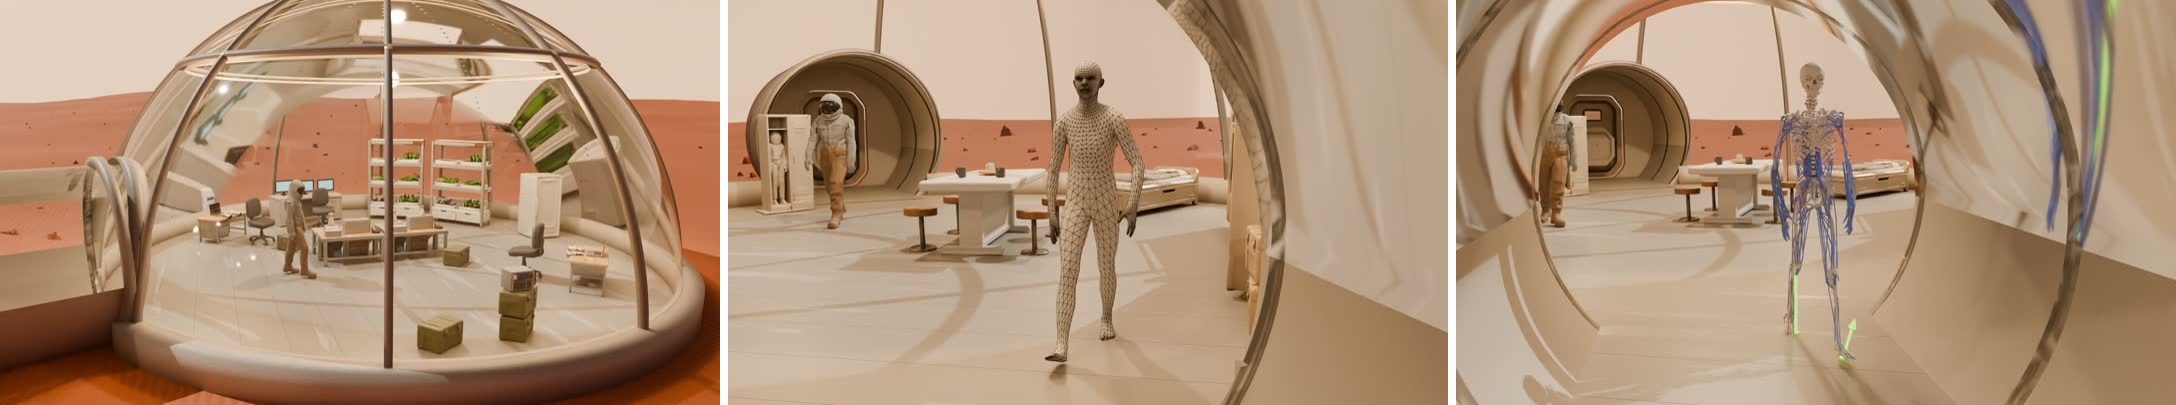
\includegraphics[width=1\linewidth,height=\textheight,keepaspectratio,alt={The peel at the end of the camp film: the player model (left), its SOMA body (centre) and its MyoFullBody sim body with its muscles and a ground reaction force arrow under the standing foot (right), walking through the tunnel between the two domes.}]{figures/peel.jpg}
\caption{The peel at the end of the camp film: the player model (left), its SOMA body (centre) and its MyoFullBody sim body with its muscles and a ground reaction force arrow under the standing foot (right), walking through the tunnel between the two domes.}
\end{figure}

\section{Results: four places}\label{results-four-places}

The creator chose four places from the first environment to rebuild: camp, two glass domes on Mars joined by a tunnel; campgrounds, the open site around them with a lander, a drilling rig and a mast; stairwell, a cut-away switchback stair in a residential block; and street, a rainy night street leading to a launch plaza. They are the three places that carried walkers in the first environment and the outdoor place that had read best under the old method. Figure 1 shows each concept beside its final render, and Table 1 summarises the scenes.

\begin{table}[tbp]
\centering\small
\caption{The four places. Objects checked and faults are from the final physics-readiness check of each scene, including its MuJoCo settle. Critic scores are the building agent's own judgement of its round-5 renders against the concept, out of 10; the old method's reviewing agents gave the same places 2, 4, 1 and 1. Films are 1920 by 1080 at 24 frames per second.}
\begin{tabular}{@{}lrrrlrr@{}}
\hline
Place & Objects & Faults & Concept view & Other views & Walkers & Film \\
\hline
camp & 711 & 0 & 7/10 & 6/10 insides & 2 & 29 s \\
campgrounds & 369 & 0 & 7/10 & 6/10 eye height & 3 & 34 s \\
stairwell & 61 & 0 & 4/10 & 6/10 insides & 2 & 24.5 s \\
street & 888 & 0 & 6/10 & 6/10 eye, 5/10 wide & 6 & 19 s \\
\hline
\end{tabular}
\end{table}

\textbf{Against the concepts.} By the critic's own scores, camp and campgrounds reach 7 out of 10 in the concept's view, street 6 and stairwell 4, against 2, 4, 1 and 1 for the same places under the per-picture method. The scores come from vision models on both sides, the old ones from reviewing agents and the new ones from the building agent's critic, and neither is a human rating; the comparison shows a change of scale rather than a calibrated measure. The renders in Figure 1 support it: the camp's two domes, their tunnel and their furnishing, the campgrounds' layout around the lander, the stairwell's cut-away flights and the street's lanterns, barriers and rain stand where the concepts place them. The critic's remaining notes are concrete. In camp everything is a pale beige and the lockers do not read as suit lockers, in campgrounds the sand ripples are too even and the sky is flat, the stairwell's view shows the building from outside rather than as the concept's cut-away and has no surroundings, and the street has boxy fronts with repeated windows and a garbled cafe sign. The street's late rain and its blotchy walls were traced to the renderer rather than to the scene, since the review's 16 samples denoised a lamp-lit haze into blotches, and reviews of places with haze now render at the films' 64 samples.

\textbf{Physics.} All four final scenes pass the physics-readiness check with no fault, including the MuJoCo settle of every prop: 711 objects in camp with its scattered rocks, 369 in campgrounds, 61 in the stairwell and 888 in the street. The check found real faults on the way, which were corrected at their source rather than tolerated. A laptop on a desk with a raised back fell 4.9 m through the desk because the settle had left out what held it, a walker's route through a loop collapsed to zero length when its legs were straightened as one path, rocks bedded deeper than 10 cm were read as unsupported, and the tunnel's skin had to be rounded to 96 points before it stopped reading as a polygon from inside.

\textbf{Walkers.} Thirteen walkers were routed and generated in the four places (Table 2, Figure 4). Twelve stay within 6.8 cm of their routes and keep at least 0.48 m from every upright solid. Eleven keep their planted feet within the 2 cm skate limit as Kimodo made them, and one street walker skates 2.9 cm; as played in the scene, foot skate reaches up to 2.9 cm for these twelve. The stairwell woman, who climbs the stair, is the exception on every measure. She strays 18 cm from her route, skates 3.6 cm in Kimodo's output and 4.7 cm as played, and passes within 0.31 m of a solid.

\begin{table}[tbp]
\centering\small
\caption{Walker measures per place, as ranges over its walkers: foot skate as Kimodo made the clip and as played in the scene, the hips' distance off the route, the least clearance from an upright solid, the peak residual force against its limit (2 percent of the body's weight under the place's gravity, Mars for camp and campgrounds, Earth for the others) and the share of frames within both residual limits.}
\begin{tabular}{@{}lrrrrrrr@{}}
\hline
 & & \multicolumn{2}{c}{Skate (cm)} & Off route & Clearance & Peak residual & Frames \\
Place & Walkers & Kimodo & played & (cm) & (m) & N (limit) & within \\
\hline
camp & 2 & 1.0--1.9 & 2.5--2.9 & 4.0--5.7 & 0.48 & 81--95 (5.7) & 74--87\,\% \\
campgrounds & 3 & 1.5--1.7 & 2.3--2.9 & 4.0--4.7 & 0.76 & 92--263 (5.6--5.7) & 56--82\,\% \\
stairwell, man & 1 & 1.7 & 1.6 & 4.0 & 0.73 & 597 (15.0) & 60\,\% \\
stairwell, woman & 1 & 3.6 & 4.7 & 18.0 & 0.31 & 1368 (15.0) & 39\,\% \\
street & 6 & 1.3--2.9 & 1.3--2.9 & 4.2--6.8 & 0.53 & 13--632 (14.9--15.2) & 79--98\,\% \\
\hline
\end{tabular}
\end{table}

\begin{figure}
\centering
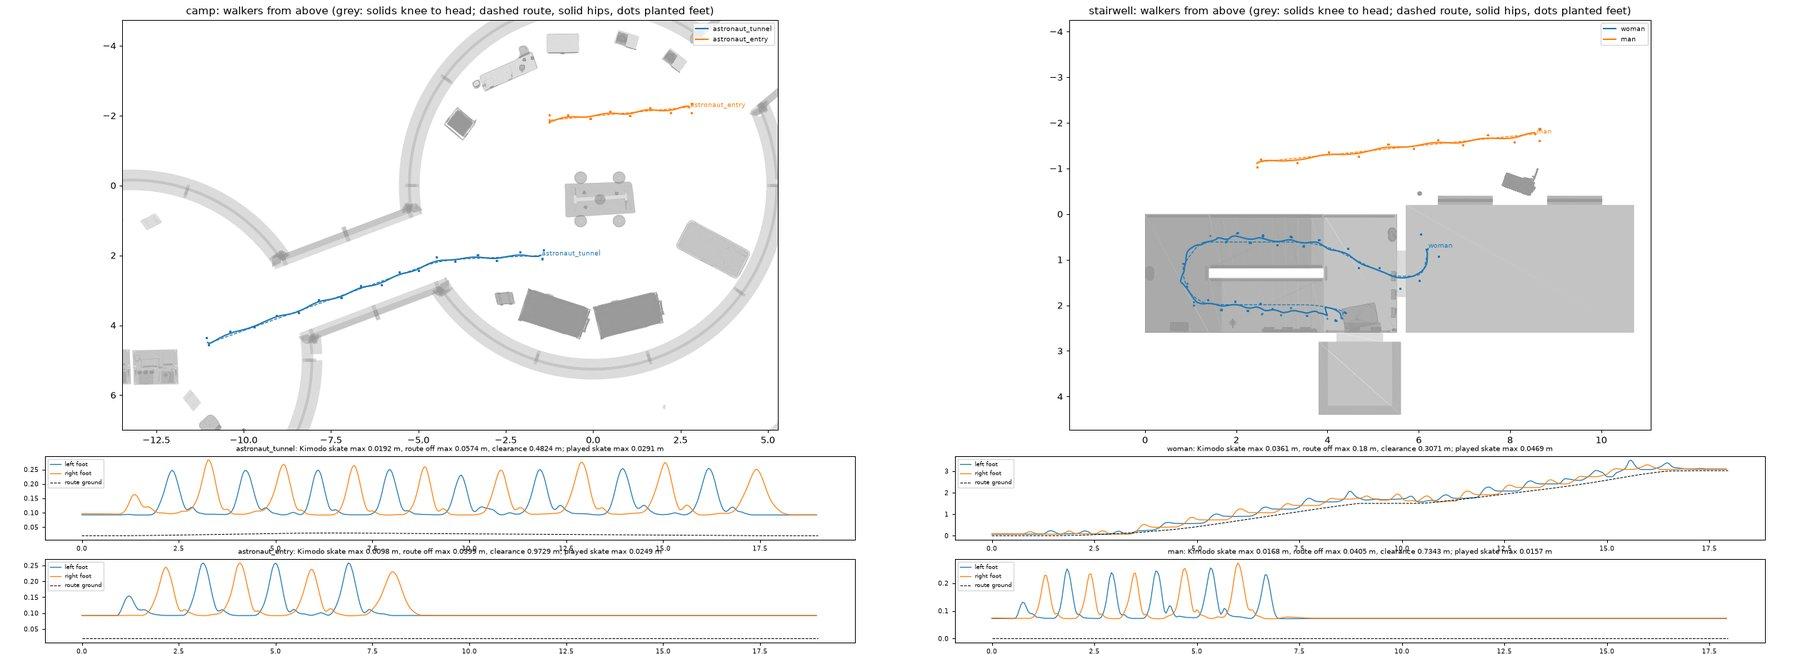
\includegraphics[width=1\linewidth,height=\textheight,keepaspectratio,alt={Walkers from above in camp (left) and the stairwell (right): grey footprints of the solids between knee and head, each walker's route dashed and its hips solid, planted feet as dots, with each walker's foot heights over time beneath. The stairwell woman's route climbs the switchback flights, and her feet follow the rising route ground.}]{figures/routes.jpg}
\caption{Walkers from above in camp (left) and the stairwell (right): grey footprints of the solids between knee and head, each walker's route dashed and its hips solid, planted feet as dots, with each walker's foot heights over time beneath. The stairwell woman's route climbs the switchback flights, and her feet follow the rising route ground.}
\end{figure}

\textbf{The residual check fails.} No walker's sim body passes the residual check over the whole clip. The best, a street walker, holds its force within the limit (13 N against 15.2 N) but not its moment (13.4 against 7.4 N m). In camp the peak residual force is 95 N against a limit of 5.7 N, while 74 to 87 percent of frames lie within both limits and the mean force is 2 to 3 N, so the failure lies in short peaks rather than throughout. The stairwell is far worse. The woman's peak reaches 1,368 N against a 15 N limit with only 39 percent of frames within, and in her film her sim body sinks about 17 cm. Section 6 discusses what this means.

\textbf{Films.} Each place's film is rendered at 1920 by 1080 and ends with its peel (Figure 5). The camp film had a final polishing round, in which its walkers walk for the whole film and the peel shows the sim body's muscles and a readable ground reaction force arrow. The other three show open faults. In campgrounds the force arrows are faint, four astronaut figures stand still and one walker starts 4.5 s late, the stairwell's man stops after 7.5 s, and in the street the peel faces the plaza's flat backdrop and most sim bodies have no centre of pressure from which to draw an arrow.

\begin{figure}
\centering
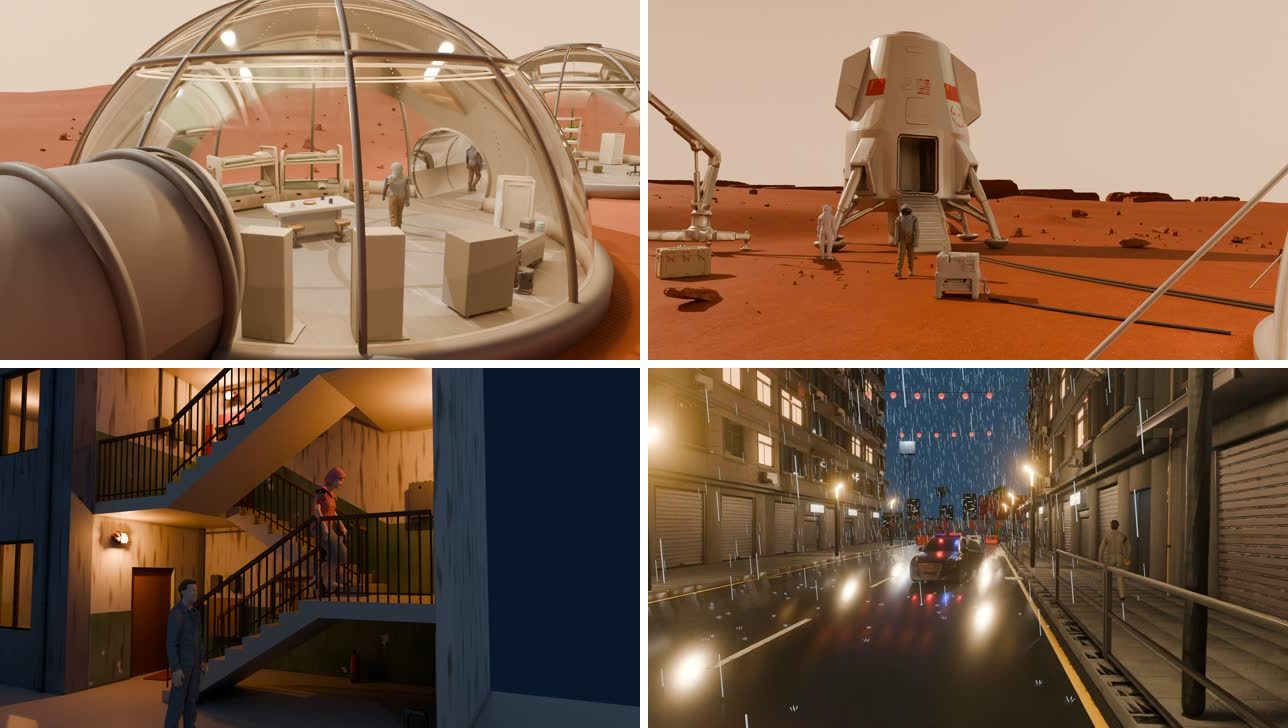
\includegraphics[width=1\linewidth,height=\textheight,keepaspectratio,alt={Frames from the four films: camp (top left), campgrounds (top right), stairwell (bottom left) and street (bottom right), each at about a third of its length.}]{figures/films.jpg}
\caption{Frames from the four films: camp (top left), campgrounds (top right), stairwell (bottom left) and street (bottom right), each at about a third of its length.}
\end{figure}

\textbf{Costs.} The four films were rendered on rented cloud graphics cards for about EUR 17. Everything else in this section was free. The building, the checks, the SAM 3 split, the TRELLIS.2 props, the walkers' Kimodo pieces and their sim bodies all ran on the creator's own computer with one 16 GB card. A TRELLIS.2 prop takes about three minutes of that card, against about EUR 0.22 (EUR 0.39 at the high estimate) for a model from the earlier paid picture-made route.

\section{Limitations and future work}\label{limitations-and-future-work}

\textbf{The residual.} A residual far above its limit means that the motion, as generated, needs a force that neither the ground nor the body supplies. The clips are kinematically clean, with little skate and close route following, and yet they are not dynamically consistent on their peaks, and on the stair the generated climb does not fit the body that follows it. The residual is recorded and never applied, so the failure is visible rather than hidden, but the walkers cannot yet be offered as physically valid motion. The stairwell woman also fails on route, skate and clearance, which points to the climb pieces and their joins rather than to the solver alone.

\textbf{Judgement.} Every score against a concept in this paper comes from a vision model, and a single creator decides what passes. Agents judge their own scenes unreliably \citep{li2026lego}, and the building agent's critic is not independent of the agent that built the scene. A human study of concept fidelity, and independent judges in the tournament with their scores kept as a record, are needed before the scores can carry weight beyond the change of scale shown here.

\textbf{Look and scope.} The scenes are not photoreal. Surfaces are clean and often pale, repeated windows and kit pieces show, the stairwell lacks its surroundings and signs are illegible. Four places were built, with walkers on Earth and Mars only. The concepts and the earlier close-ups were drawn by closed models that may change or be withdrawn. The placement itself is an agent's work under the creator's direction, so a place costs agent time rather than money, which this paper has not measured.

\textbf{Future work.} Next come the walkers' residuals, through climb pieces that fit the stair, contact in the clip generation and the solver work reported in MOTOR \citep{motor}; independent judges and a human rating of concept fidelity; the remaining places of the first environment; and the uses that SCORE was built for. A sim body that is true to the individual person, validated against measured forces, would let the same scenes yield layered training data. Each sample would pair a rendered image of a person in a complete scene with the body, its joint moments, its ground reaction forces and muscle forces, and a residual that selects only the dynamically consistent movements \citep{delp2007opensim, werling2023addbiomechanics, huo2026biohuman}.

\textbf{Disclosure.} The creator's locks, picks and decisions are his own, made in chat. Everything between them was done by coding agents, which placed every object of the four scenes, judged their renders and ran the tournament, and which wrote most of the framework's code under the author's direction: 4,211 of its 4,238 commits list a coding agent as co-author. No scene was edited by hand.

\section{Conclusion}\label{conclusion}

SCORE builds environments that a simulator can step and that their creator owns. Deriving a scene from its concept through a chain of readings and written plans failed, scoring 2.2 out of 10 across 26 places, because the scaffolding between good models went wrong in ways that rules could not repair. Placing library pieces under a render-and-compare loop, with a physics-readiness check that refuses anything a simulator could not use, produced four places that read far closer to their concepts, with no physics fault, at a cost of about EUR 17 in rendering. Walkers route through these scenes on checked floor with clips joined into one motion, and each carries a musculoskeletal sim body whose residual shows honestly where generated motion is not yet physical. That residual is now the open problem. Once generated movement in complete, simulable scenes passes it, such scenes can supply training data that recorded measurement cannot provide at scale.


\bibliographystyle{unsrtnat}
\bibliography{refs}


\end{document}
